\documentclass[polish,12pt]{aghthesis}
\usepackage[utf8x]{inputenc}
\usepackage{url}
\usepackage{graphicx}
\usepackage{hyperref}
\usepackage{minted}
\usepackage{float}
\usepackage{perpage}

\MakePerPage{footnote}

\graphicspath{ {./images/} }

\author{Piotr Szczygieł}

\titlePL{Gra typu Capture-The-Flag\\ oparta o reverse engineering}
\titleEN{Capture-The-Flag game based on reverse engineering}

\fieldofstudy{Informatyka}

\supervisor{dr inż.\ Łukasz Faber}

\date{\the\year}

\begin{document}

\maketitle

\tableofcontents
\newpage

\section{\SectionTitleProjectVision}
\label{sec:cel-wizja}

\subsection{Wprowadzenie}

Gra typu Capture-the-Flag jest to rodzaj zawodów z ogólnie pojętego
bezpieczeństwa komputerowego. Ich celem zwykle jest edukacja uczestników
o zabezpieczeniach systemów oraz możliwość pokazania im jak reagować
na wypadek wystąpienia rzeczywistych ataków. Zawody takie podzielone są zazwyczaj
na poszczególne zadania z różnych kategorii. Aby rozwiązać takie zadanie należy
znaleźć ,,flagę'', którą następnie podaje się w interfejsie udostępnionym przez
organizatora zawodów. Flagą w tym wypadku jest ciąg znaków, który możemy uzyskać
poprzez rozwiązanie zadania. Przykładowo w najprostszych zadaniach
z dziedziny eksploitacji stron internetowych, flagę możemy znaleźć klikając
"Pokaż źródło strony" w przeglądarce internetowej.

\begin{figure}[ht]
    \centering
    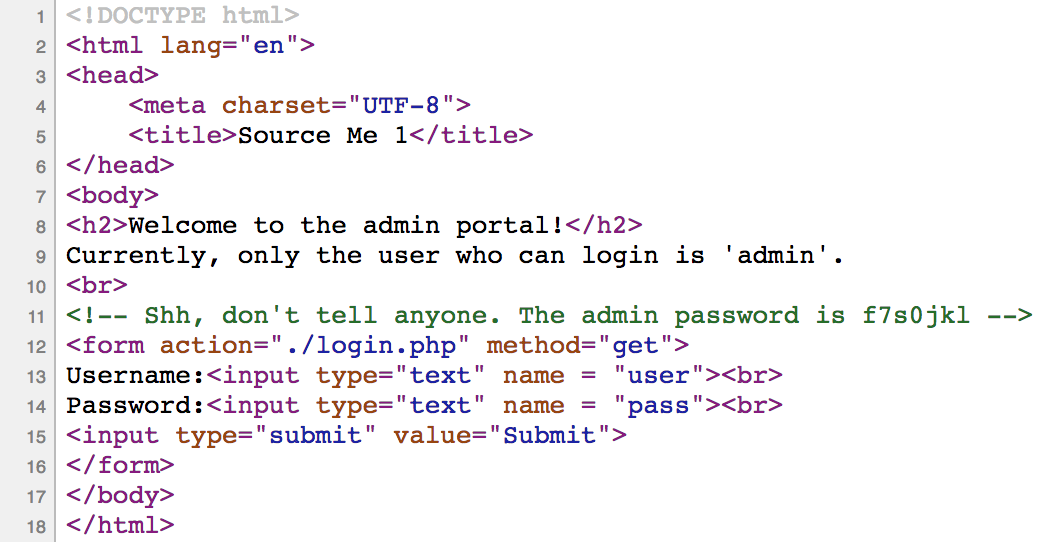
\includegraphics[width=10cm]{flag_page_source}
    \caption{Flaga \textbf{f7s0jkl} ukryta w źródle strony internetowej}
    \label{fig:flag_page_source}
\end{figure}

W tej pracy zaprezentowana będzie jednak grę oparta
wyłącznie o Reverse Engineering (ang. Inżynieria Wsteczna).
Inżynieria wsteczna oprogramowania może odbywać się na różne sposoby.
Może to być przykładowo wykorzystanie tzw. snifferów do analizy protokołów
komunikacyjnych aplikacji internetowej. W tym wypadku będzie ona jednak
zazwyczaj oznaczała proces analizy programu, aby zrozumieć co robi
oraz w jaki sposób. Przedstawione zadania można by też podpiąć do kategorii
eksploitacji binarnej (ang. Binary Exploitation), która w pewny sposób pokrywa
się z zagadnieniami Reverse Engineeringu. Jest to mianowicie proces
wykorzystywania niedoskonałości programów w celu zmuszenia ich do zrobienia
czegoś, czego w normalnej sytuacji nie powinny robić. Te dwie kategorie pokrywają
się ze sobą, ponieważ zazwyczaj nie jest możliwe rozwiązanie zadania z kategorii
eksploitacji binarnej, bez wykorzystania do tego inżynierii wstecznej. \pagebreak

Produktem końcowym będzie zbiór kilku zadań udostępniony na platformie webowej.
Platforma sama w sobie nie jest niczym specjalnym, udostępnia jedynie takie powszechne
funkcjonalności jak rejestracja użytkowników, ranking najlepszych graczy,
pobieranie zadań oraz interfejs umożliwiający wprowadzanie znalezionych
flag. Z tego względu użyta zostanie gotowa platforma CTFd\footnote{
Informacje o platformie CTFd dostępne pod adresem \url{https://ctfd.io/}}.
Użycie takiego gotowego rozwiązania pozwoli w pełni skupić się na samych zadaniach,
a ominąć takie kwestie jak np. gracze łamiący zabezpieczenia platformy.

\begin{figure}[ht]
    \centering
    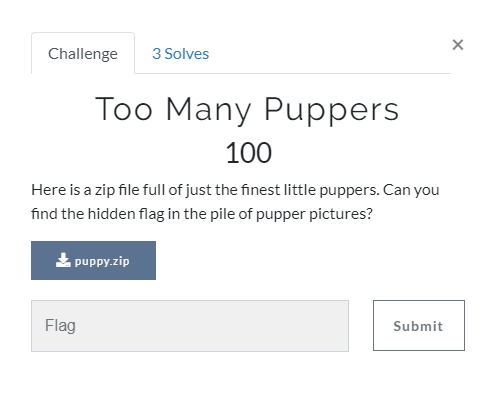
\includegraphics[width=10cm]{ctfd}
    \caption{Przykładowe zadanie na stronie demonstracyjnej CTFd}
    \label{fig:ctfd}
\end{figure}

W tej pracy opisany zostanie zarówno proces tworzenia poszczególnych zadań,
jak i przykładowe ich rozwiązania. Użyte zostało słowo "przykładowe", ponieważ
w takiej kategorii jak Binary Exploitation / Reverse Engineering liczba sposobów
na rozwiązanie danego zadania jest ograniczona jedynie przez wyobraźnie uczestnika.
Nie ograniczymy się również do korzystania ciągle z tych samych narzędzi.
Pokazane zostaną różnorodne podejścia do analizy i rozwiązywania wyzwań.
Zadania będą tworzone z zamiarem zachowania rosnącego stopnia trudności.
Na początku uczestnik będzie miał szansę rozwiązać proste zadania,
zachęcające go do dalszej rozgrywki. Finalne zadania powinny stanowić wyzwanie
nawet dla doświadczonych graczy. \pagebreak

\subsection{Dostępne platformy}

Aktualnie istnieje wiele różnych zawodów CTF online. Jednym z popularniejszych
jest \mbox{picoCTF}\footnote{
Zawody picoCTF dostępne pod adresem \url{https://picoctf.com/}}.
Można tam wejść kiedykolwiek, zalogować się i zająć się rozwiązywaniem problemów.

\begin{figure}[ht]
    \centering
    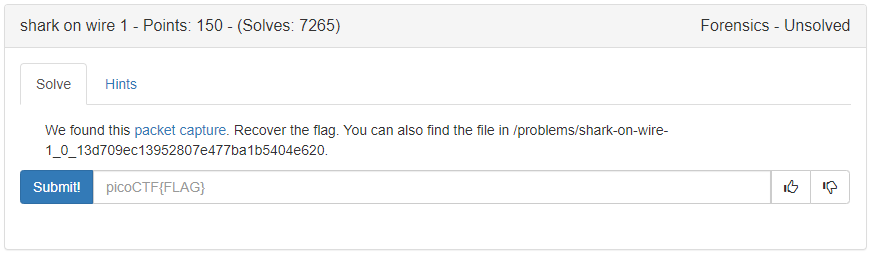
\includegraphics[width=15cm]{picoctf}
    \caption{Zadanie z kategorii Forensics na stronie picoCTF}
    \label{fig:picoctf}
\end{figure}

Główną motywacją do napisania tej pracy jest fakt, że strony tego typu często skupiają
się na zadaniach w takich kategoriach jak Forensics czy Web Exploitation.
Mnie natomiast bardzo interesuję temat inżynierii wstecznej i chciałem
przygotować wyzwania oparte o zadania tylko z tej kategorii.

\subsection{Języki programowania i narzędzia}

Zadania będą tworzone w języku C. Jest to powszechnie znany język, który
z wyłączoną zbyt agresywną optymalizacją ze strony kompilatora, generuje
w miarę przewidywalny kod maszynowy. Zaletą tego jest to, że narzędzia
do debugowania, deasemblacji oraz wykonywania innych analiz programów
dobrze radzą sobie z takimi plikami. Dzięki temu język ten
zapewni nam kontrolę nad tym w jakim stopniu graczowi ułatwimy
lub utrudnimy rozgrywkę. W celu zapewnienia większej różnorodności
środowisk korzystać będziemy zarówno z systemu Windows jak i Linux.

Do rozwiązywania zadań posłużymy się różnorodnymi rodzajami narzędzi.
Poczynając od linuksowych programów linii poleceń takich jak \mintinline{bash}{strings}
czy \mintinline{bash}{gdb}, pisania własnych narzędzi w języku \emph{Python},
czy w końcu korzystając z pełnoprawnych narzędzi z interfejsem graficznym takich
jak \emph{Cutter}, czy używana przez NSA \emph{Ghidra}.

\clearpage

\section{\SectionTitleScope}
\label{sec:zakres-funkcjonalnosci}

\subsection{Platforma}

Do interfejsu webowego skorzystamy z gotowej platformy CTFd.
Finalny produkt będzie dostępny pod adresem
\href{https://ctf.szczygiel.dev}{https://ctf.szczygiel.dev}.
Strona postawiona będzie na prywatnym serwerze VPS. Platforma będzie
uruchomiona w środowisku docker, a wystawiona do świata będzie poprzez serwer Caddy\footnote{
Serwer Caddy: \url{https://caddyserver.com/}},
który w prosty sposób zapewni nam HTTPS, dzięki organizacji Let's Encrypt\footnote{
Organizacja Let's Encrypt: \url{https://letsencrypt.org/}}.

\subsection{Użytkownicy}

Użytkownikiem systemu będzie każda osoba zainteresowana rozwiązywaniem
tego rodzaju zadań. Może to być zarówno ktoś kształcący się lub pracujący
w dziale informatycznym, jak i osoba dla której jest to jedynie hobby.

Wszystkie gotowe zadania zostaną wrzucone na platformę, dzięki czemu
każda zainteresowana osoba będzie mogła spróbować swoich sił.

\clearpage

\subsection{Prezentacja interfejsu użytkownika}

\begin{figure}[ht]
    Pierwsze co zobaczy każdy użytkownik wchodzący na platformę, to strona główna.
    Będzie z niej można przejść do reszty podstron, takich jak logowanie, rejestracja,
    wylogowanie, spis graczy, tabela wyników oraz lista dostępnych zadań.

    \vspace{1cm}

    \centering
    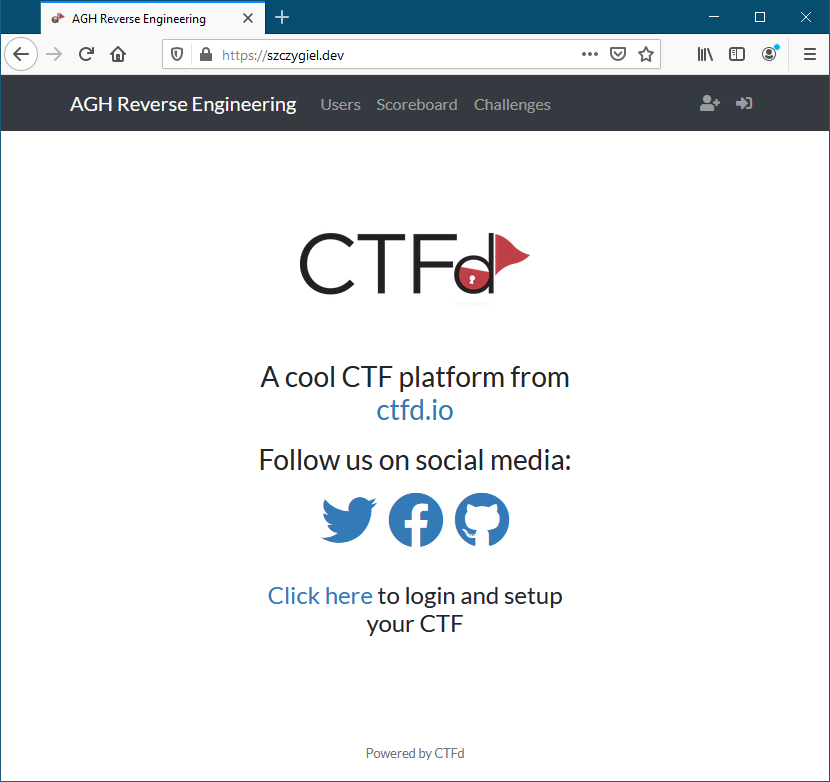
\includegraphics[width=14cm]{szczygiel_dev}
    \caption{Strona głowna platformy CTF}
    \label{fig:szczygiel_dev}
\end{figure}

\begin{figure}[ht]
    Poniżej przedstawiony jest interfejs rejestracji nowego użytkownika.
    Nie będzie to nic skomplikowanego -- wystarczy podać login, email oraz hasło.

    \vspace{1cm}

    \centering
    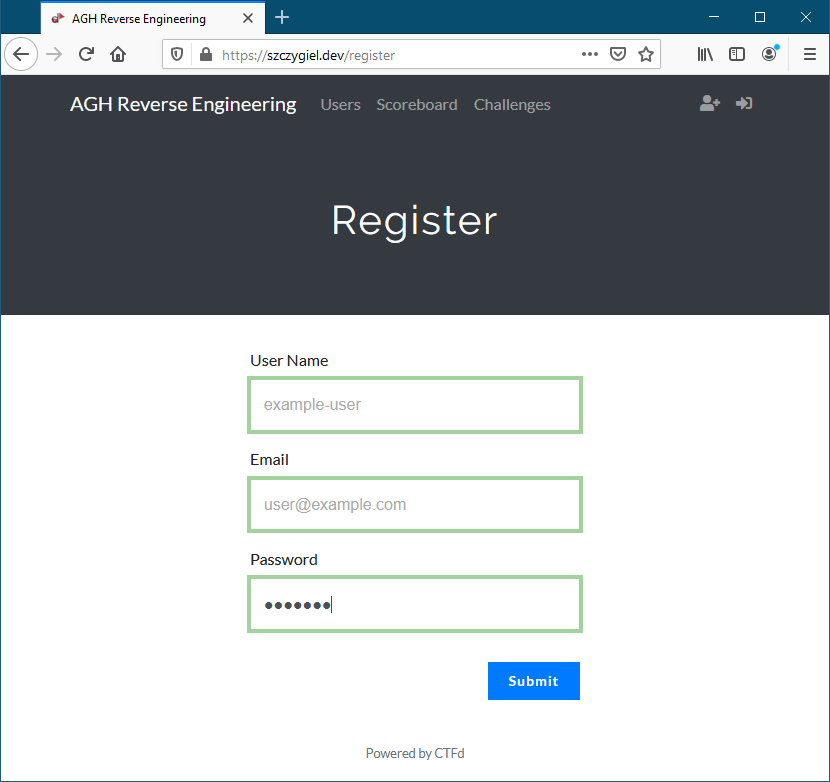
\includegraphics[width=14cm]{szczygiel_dev_register}
    \caption{Rejestracja nowego użytkownika}
    \label{fig:szczygiel_dev_register}
\end{figure}

\begin{figure}[ht]
    Jeśli użytkownik posiada konto to będzie się mógł na nie zalogować.

    \vspace{1cm}

    \centering
    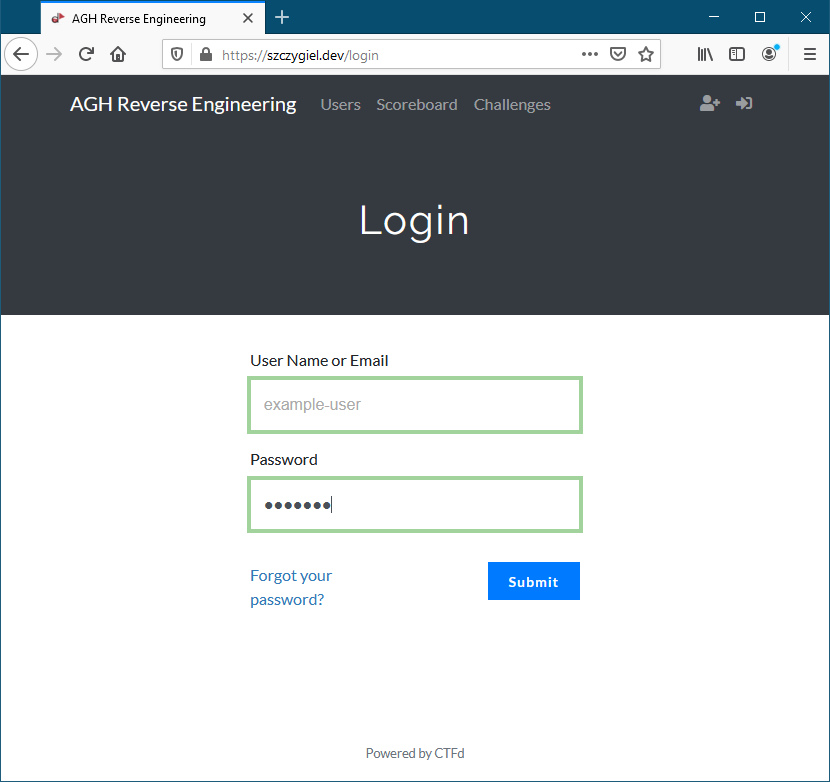
\includegraphics[width=14cm]{szczygiel_dev_login}
    \caption{Panel logowania dla istniejącego użytkownika}
    \label{fig:szczygiel_dev_login}
\end{figure}

\begin{figure}[ht]
    Będąc zalogowanym, można wybrać zadanie które ma się ochote rozwiązać.

    \vspace{1cm}

    \centering
    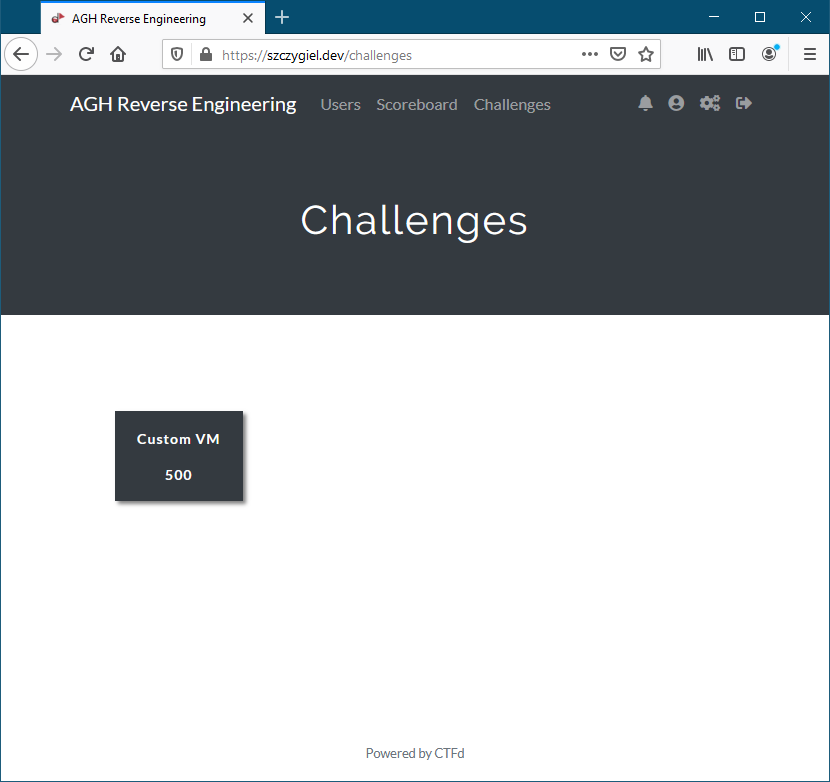
\includegraphics[width=14cm]{szczygiel_dev_challenges}
    \caption{Wybór zadania do rozwiązania}
    \label{fig:szczygiel_dev_challenges}
\end{figure}

\begin{figure}[ht]
Po wybraniu interesującego nas zadania, można pobrać dostarczony plik,
    a następnie po rozwiązaniu zadania wprowadzić prawidłową (lub nie) flagę.

    \vspace{1cm}

    \centering
    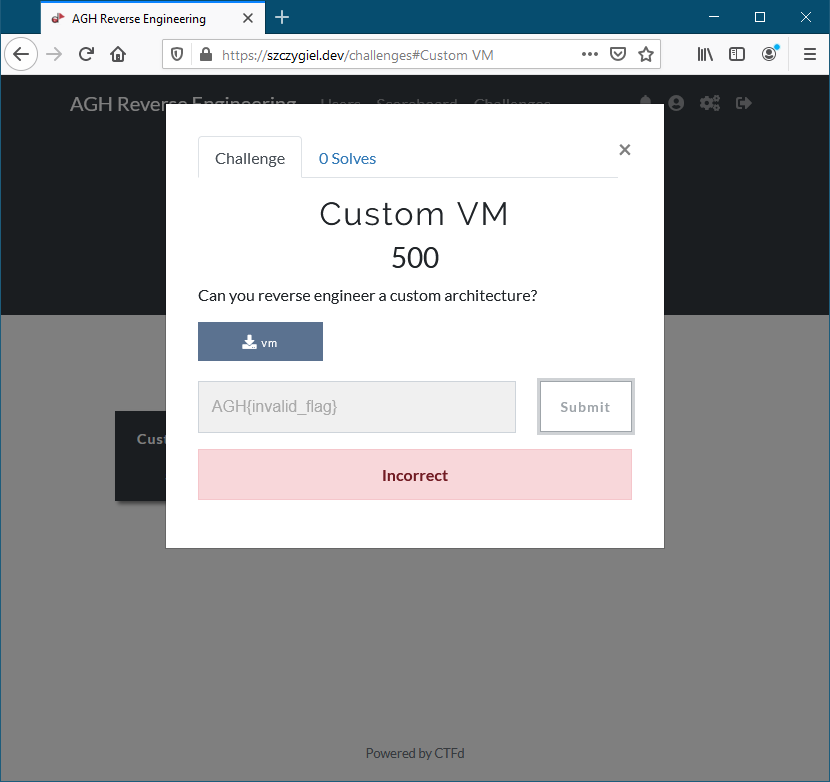
\includegraphics[width=14cm]{szczygiel_dev_incorrect}
    \caption{Interfejs zadania oraz wprowadzenie nieprawidłowej flagi}
    \label{fig:szczygiel_dev_incorrect}
\end{figure}

\begin{figure}[ht]
    Po wprowadzeniu prawidłowej flagi otrzymamy stosowny komunikat.
    Można również zauważyć, że zadanie w tle zmieniło kolor na zielony.

    \vspace{1cm}

    \centering
    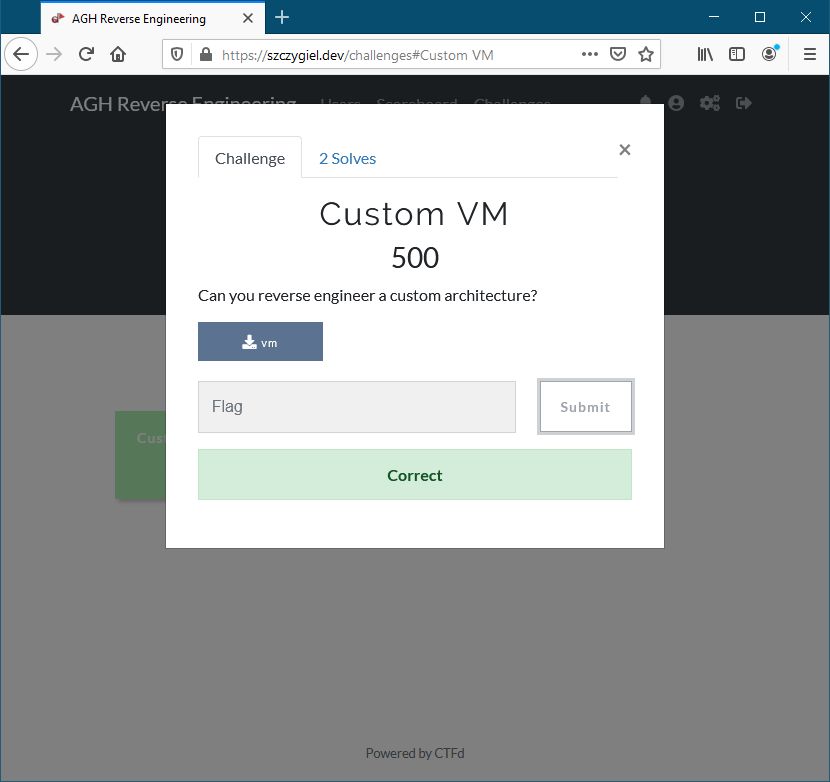
\includegraphics[width=14cm]{szczygiel_dev_correct}
    \caption{Efekt wprowadzenia prawidłowej flagi}
    \label{fig:szczygiel_dev_correct}
\end{figure}

\begin{figure}[ht]
    Dostępna jest również lista zarejestrowanych użytkowników.
    Można wejść w profil każdego użytkownika i zobaczyć jego postępy.

    \vspace{1cm}

    \centering
    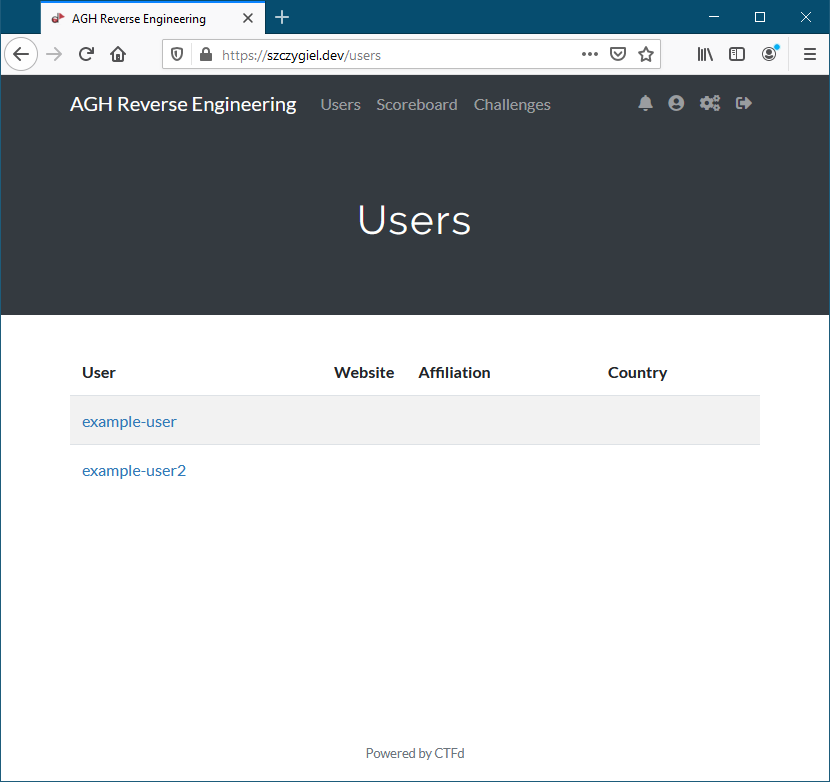
\includegraphics[width=14cm]{szczygiel_dev_users}
    \caption{Spis zarejestrowanych użytkowników}
    \label{fig:szczygiel_dev_users}
\end{figure}

\begin{figure}[ht]
Wchodząc na profil użytkownika można zobaczyć o nim różne informacje.
Jest to przede wszystkim rozkład prawidłowych oraz nieprawidłowych
    wprowadzeń flag oraz wykres posiadanych punktów w czasie.
    Na dole widzimy również wszystkie rozwiązane przez użytkownika zadania.

    \vspace{1cm}

    \centering
    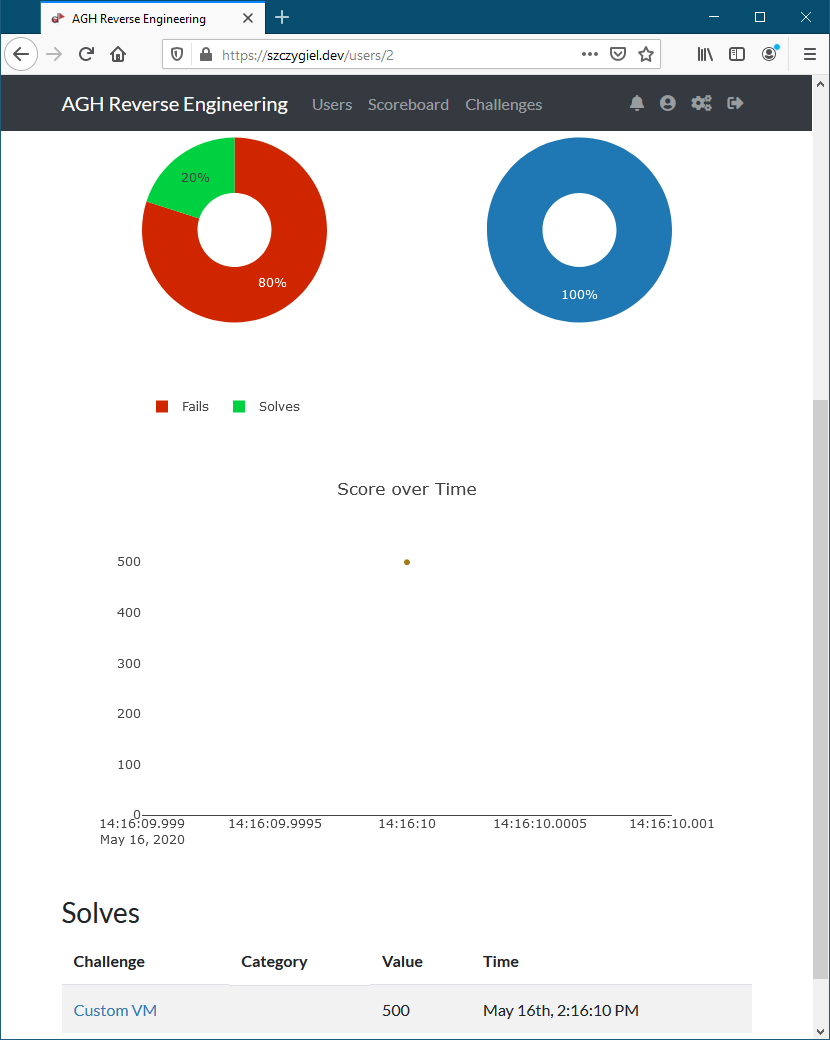
\includegraphics[width=14cm]{szczygiel_dev_user_info}
    \caption{Szczegóły postępów konkretnego użytkownika}
    \label{fig:szczygiel_dev_user_info}
\end{figure}

\begin{figure}[ht]
    Każdy użytkownik może również zmienić oraz dodać informację o sobie.
    Będzie mógł zmienić nazwę użytkownika, email, hasło, oraz dodać
    takie szczegóły jak strona internetowa, firma dla której pracuję czy kraj pochodzenia.

    \vspace{1cm}

    \centering
    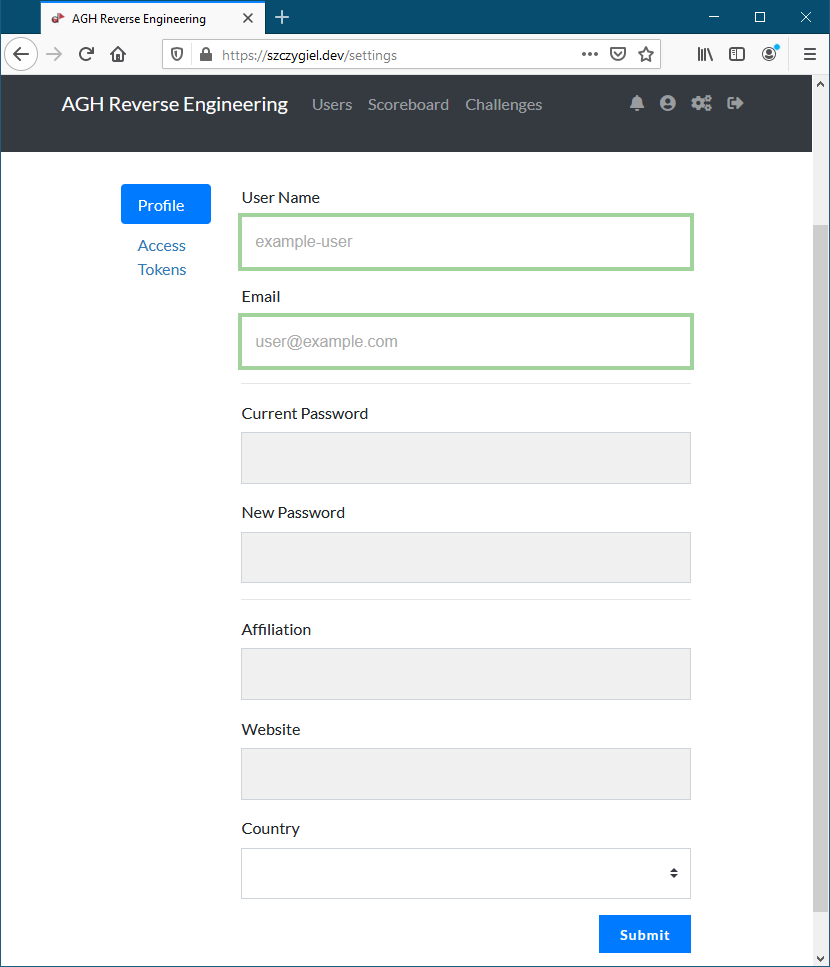
\includegraphics[width=14cm]{szczygiel_dev_settings}
    \caption{Edycja profilu użytkownika}
    \label{fig:szczygiel_dev_settings}
\end{figure}

\clearpage

\section{\SectionTitleRealizationAspects}
\label{sec:wybrane-aspekty-realizacji}

W tym rozdziale przedstawione zostaną sposoby tworzenia poszczególnych zadań.
Warto dodać również, że zawarte w opisach flagi są przykładowe i w formacie
\emph{AGH\{nazwa-zadania\}}, aby nie wyjawiać prawdziwych flag użytych w rozgrywce.
Przykładowe rozwiązania zadań znajdują się w rozdziale 5 -- \nameref{sec:wyniki-projektu}.

\subsection{Zadanie 100-simple}

Pierwszym zadaniem jest odnalezienie flagi wprost umieszczonej
w pliku wykonywalnym jako ciąg znaków.
Zadanie to służyć ma jako pewnego rodzaju rozgrzewka i powinno być stosunkowo
proste do rozwiązania nawet przez kompletnie początkujących zawodników.
Poniżej przedstawiona uproszczona\footnote{Uproszczona, czyli zawierająca jedynie
najważniejsze fragmenty kodu, pozbawiona sprawdzania błędów, definicji funkcji
pomocniczych, załączania nagłówków itp.} wersja kodu źródłowego.

\begin{minted}{c}
int main()
{
    char input[64];

    printf("Enter the flag: ");
    fgets(input, sizeof(input), stdin);
    input[strlen(input) - 1] = '\0';

    if (strcmp(input, "AGH{100-simple}") == 0) {
        printf("Correct flag!\n");
    } else {
        printf("Incorrect flag!\n");
    }

    return 0;
}
\end{minted}

Jak widać program jedynie co robi, to pobiera wejście od użytkownika, a następnie
porównuje je z zapisaną na stałe w kodzie flagą. Użytkownik po inspekcji skompilowanego
pliku wykonywalnego komendą \mintinline{bash}{strings} powinien szybko zwrócić uwagę na
ciąg znaków wyglądający jak rozwiązanie tego zadania.
\clearpage

\subsection{Zadanie 200-game}

W drugim zadaniu flaga będzie odszyfrowana zaraz po uruchomieniu programu. Zadaniem
użytkownika będzie odnalezienie tej flagi poprzez modyfikacje
pliku wykonywalnego w celu zmiany zachowania programu.

Sam program będzie działać w graficznym środowisku systemu Windows.
Do obsługi okienek i innych aspektów graficznych wykorzystana została
biblioteka raylib\footnote{
Biblioteka raylib: \url{https://www.raylib.com/}}.
Poniżej przedstawiony kod programu z pominięciem funkcji \emph{decrypt\_flag}.

\begin{minted}[breaklines]{c}
bool show_flag()
{
    return false;
}

int main()
{
    if (show_flag()) {
        decrypt_flag();
    }

    SetTraceLogLevel(LOG_ERROR);
    InitWindow(460, 40, "200-game");
    SetTargetFPS(60);

    while (!WindowShouldClose()) {
        BeginDrawing();
        ClearBackground(BLACK);

        if (show_flag()) {
            DrawText((const char*)flag, 10, 10, 20, GREEN);
        } else {
            DrawText("You have not unlocked access to the flag!", 10, 10, 20, RED);
        }

        EndDrawing();
    }

    CloseWindow();
    return 0;
}
\end{minted}

Sednem całego zadania jest funkcja \emph{show\_flag}, która kontroluje czy rozwiązanie
ukaże się użytkownikowi oraz czy flaga w ogóle zostanie odszyfrowana.
Jeśli chodzi o samo szyfrowanie flagi, użyte zostało do tego narzędzie\footnote{
zerosum0x0: Obfuscated String/Shellcode Generator - Online Tool
\url{https://zerosum0x0.blogspot.com/2017/08/obfuscatedencrypted-cc-online-string.html}}
pozwalające zamienić ciąg znaków na tablice bajtów wraz z algorytmem odszyfrowującym.
Poniżej przedstawiony fragment wyniku działania takiego narzędzia.

\begin{minted}{c}
unsigned char flag[] = {
    0xa6, 0x40, 0x70, 0x2b, 0x6e, 0xed, 0x80,
    0x19, 0x36, 0xe1, 0x8a, 0xcd, 0x98, 0xa2
};

void decrypt_flag()
{
    for (unsigned int m = 0; m < sizeof(flag); ++m) {
        unsigned char c = flag[m];
        c = (c >> 0x1) | (c << 0x7);
        c ^= 0x74;
        c = -c;
        c += 0x3f;

        ...

        c ^= 0xc8;
        c = ~c;
        c = -c;
        c -= 0x51;
        flag[m] = c;
    }
}
\end{minted}

Odszyfrowanie flagi korzystając z kodu zdekompilowanej funkcji \emph{decrypt\_flag} jest możliwe,
jednak użytkownik powinien sobie dużo szybciej poradzić z rozwiązaniem zadania prostszymi
sposobami.
\clearpage

\subsection{Zadanie 300-strcmp}

Trzecie zadanie będzie połączeniem dwóch wcześniejszych.
Poniżej przedstawiona uproszczone wersja kodu źródłowego, bez funkcji \emph{decrypt\_flag}.

\begin{minted}[breaklines]{c}
int main()
{
    decrypt_flag();

    char input[64];

    printf("Enter the flag: ");
    fgets(input, sizeof(input), stdin);
    input[strlen(input) - 1] = '\0';

    if (strcmp(input, (char*)flag) == 0) {
        printf("Correct flag!\n");
    } else {
        printf("Incorrect flag!\n");
    }

    return 0;
}
\end{minted}

Jak widać kod jest taki sam jak w zadaniu pierwszym, jedynie z tą różnicą, że
flaga zamiast zapisana w kodzie w jawny sposób, jest odszyfrowywana zaraz po uruchomieniu
programu -- podobnie jak w zadaniu drugim.
\clearpage

\subsection{Zadanie 400-decrypt}

Czwarte zadanie będzie zawierało funkcje szyfrującą wejście użytkownika, a następnie to wejście będzie
porównywane z wcześniej zaszyfrowaną flagą. Zadaniem użytkownika będzie przykładowo napisanie skryptu
odwracającego działanie funkcji szyfrującej i uruchomienie go podając na wejście zaszyfrowaną flagę
wyciągniętą z pliku wykonywalnego.

Funkcja szyfrującą będzie dzieliła się na dwa etapy. Pierwszym etapem będzie użycie prostego
szyfru Cezara z przesunięciem 13 -- zwanym także ROT13. Drugi etap będzie to prosty szyfr XOR
z użyciem 4 bajtowego klucza. Poniżej przestawiony uproszczony kod funkcji \emph{main} programu.

\begin{minted}[breaklines]{c}
int main()
{
    char input[64];
    printf("Enter the flag: ");
    fgets(input, sizeof(input), stdin);

    int length = strlen(input) - 1;
    input[length] = '\0';

    if (length == sizeof(flag)) {
        encrypt(input, length);

        if (memcmp(input, flag, length) == 0) {
            printf("Correct flag!\n");
            return 0;
        }
    }

    printf("Incorrect flag!\n");
    return 0;
}
\end{minted}

Jak widać główny kod programu jest bardzo prosty i nie różni się specjalnie od poprzednich zadań.
\clearpage

Poniżej przedstawiona zostanie funkcja szyfrująca \emph{encrypt}.

\begin{minted}{c}
void encrypt(char* input, int length)
{
    for (int i = 0; i < length; ++i) {
        char c = input[i];

        if (c >= 'A' && c <= 'Z') {
            if (c + 13 <= 'Z')
                input[i] = c + 13;
            else
                input[i] = c - 13;
        } else if (c >= 'a' && c <= 'z') {
            if (c + 13 <= 'z')
                input[i] = c + 13;
            else
                input[i] = c - 13;
        }
    }

    char key[] = { 0xde, 0xad, 0xbe, 0xef };
    int k = 0;

    for (int i = 0; i < length; ++i) {
        input[i] ^= key[k];
        k = (k + 1) % sizeof(key);
    }
}
\end{minted}

Pierwsza część szyfrowania, czyli ROT13, przechodzi po kolei po każdym znaku na wejściu i jeśli jest to litera,
to przesuwa ją o 13 w lewo albo 13 w prawo. Druga część to prosty szyfr XOR z kluczem \emph{0xde, 0xad, 0xbe, 0xef}.
Program przechodzi po kolei po każdym znaku i wykonuje operacje XOR z kolejnymi bajtami klucza. Jeśli dojdziemy
do ostatniego bajta klucza -- wracamy z powrotem do pierwszego bajtu.

\clearpage
Ostatnim krokiem jest wygenerowanie tablicy \emph{flag}. Tworzymy nowy program - \emph{generate}, zawierający
zmodyfikowaną funkcję \emph{main}, która zwróci nam finalną zawartość tablicy \emph{flag}.
Poniżej przestawiony zmodyfikowany kod funkcji \emph{main} dla programu \emph{generate}.

\begin{minted}{c}
int main()
{
    char input[64];
    fgets(input, sizeof(input), stdin);

    int length = strlen(input) - 1;
    input[length] = '\0';

    encrypt(input, length);

    for (int i = 0; i < length; ++i) {
        printf("0x%02x, ", (unsigned char)input[i]);
    }

    return 0;
}
\end{minted}

Kompilujemy i uruchamiamy program, podając mu na wejście flagę, którą użytkownik będzie musiał odgadnąć.

\begin{minted}[breaklines]{text}
$ make generate
gcc -Wall -Wextra -std=c99 generate.c -o generate
$ ./generate
AGH{400-decrypt}
0x90, 0xf9, 0xeb, 0x94, 0xea, 0x9d, 0x8e, 0xc2, 0xaf, 0xdf, 0xce, 0x8a, 0xb2, 0xce, 0xd9, 0x92,
\end{minted}

Teraz możemy do głównego programu dodać definicje tablicy \emph{flag}.

\begin{minted}[breaklines]{c}
char flag[] = { 0x90, 0xf9, 0xeb, 0x94, 0xea, 0x9d, 0x8e, 0xc2, 0xaf, 0xdf, 0xce, 0x8a, 0xb2, 0xce, 0xd9, 0x92 };
\end{minted}
\clearpage

\subsection{Zadanie 500-secret-shell}

\subsection{Zadanie 600-custom-vm}

\clearpage

\section{\SectionTitleWorkOrganization}
\label{sec:organizacja-pracy}
\emph{Struktura zespołu (role poszczególnych osób), krótki opis i
    uzasadnienie przyjętej metodyki i/lub kolejności prac, planowane i
    zrealizowane etapy prac ze wskazaniem udziału poszczególnych
    członków zespołu, wykorzystane praktyki i narzędzia w zarządzaniu
    projektem.}

\clearpage

\section{\SectionTitleResults}
\label{sec:wyniki-projektu}

W tym rozdziale przedstawione zostaną przykładowe sposoby rozwiązania poszczególnych zadań.
Podobnie jak w rozdziale opisującym proces tworzenia tych zadań, znalezione
flagi są przykładowe.

\subsection{Zadanie 100-simple}

Po otworzeniu karty z pierwszym zadaniem uczestnik pobiera załączony do niego
plik -- \emph{simple}.
Na początku sprawdza z jakim rodzajem pliku ma do czynienia.

\begin{minted}[breaklines]{text}
$ file simple
simple: ELF 64-bit LSB pie executable, x86-64, version 1 (SYSV), dynamically linked, interpreter /lib64/ld-linux-x86-64.so.2, BuildID[sha1]=4bfaf13eb10701fb33b5442a8e17056253509ef1, for GNU/Linux 3.2.0, with debug_info, not stripped
\end{minted}

Jak zauważa, jest to plik wykonywalny dla 64-bitowego systemu Linux.
Uruchamia więc program, aby sprawdzić jego zachowanie.

\begin{minted}{text}
$ ./simple
Enter the flag: test
Incorrect flag!
\end{minted}

Na początku rozwiązywania każdego zadania z kategorii Reverse Engineering, warto
przejrzeć, czy plik wykonywalny nie zawiera jakiś przydatnych ciągów znaków.

\begin{minted}{text}
$ strings simple
/lib64/ld-linux-x86-64.so.2
puts
__stack_chk_fail
...
Enter the flag: 
AGH{100-simple}
Correct flag!
Incorrect flag!
...
\end{minted}

Zauważa ciekawie wyglądający ciąg znaków \emph{AGH\{100-simple\}}.
Uruchamia więc program jeszcze raz, podając mu ten ciąg znaków na wejście.

\begin{minted}{text}
$ ./simple
Enter the flag: AGH{100-simple}
Correct flag!
\end{minted}

Otrzymuje informację, że jest to prawidłowa flaga.
Po wpisaniu go na stronie zadania dowiaduje się, że jest to prawidłowe rozwiązanie.

\subsection{Zadanie 200-game}

Użytkownikowi po pobraniu oraz uruchomieniu załączonego pliku \emph{game.exe} ukazuję
się następujące okienko.

\begin{figure}[H]
    \centering
    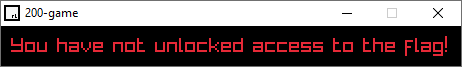
\includegraphics{200_not_unlocked}
    \caption{Okienko programu z informacją o braku dostępu do flagi}
    \label{fig:200_not_unlocked}
\end{figure}

Użytkownik otwiera plik wykonywalny w programie IDA\footnote{
Darmowa wersja programu IDA przeznaczona do użytku domowego dostępna do pobrania pod adresem 
\url{https://www.hex-rays.com/products/ida/support/download_freeware}},
aby zapoznać się z działaniem programu.

\begin{figure}[H]
    \centering
    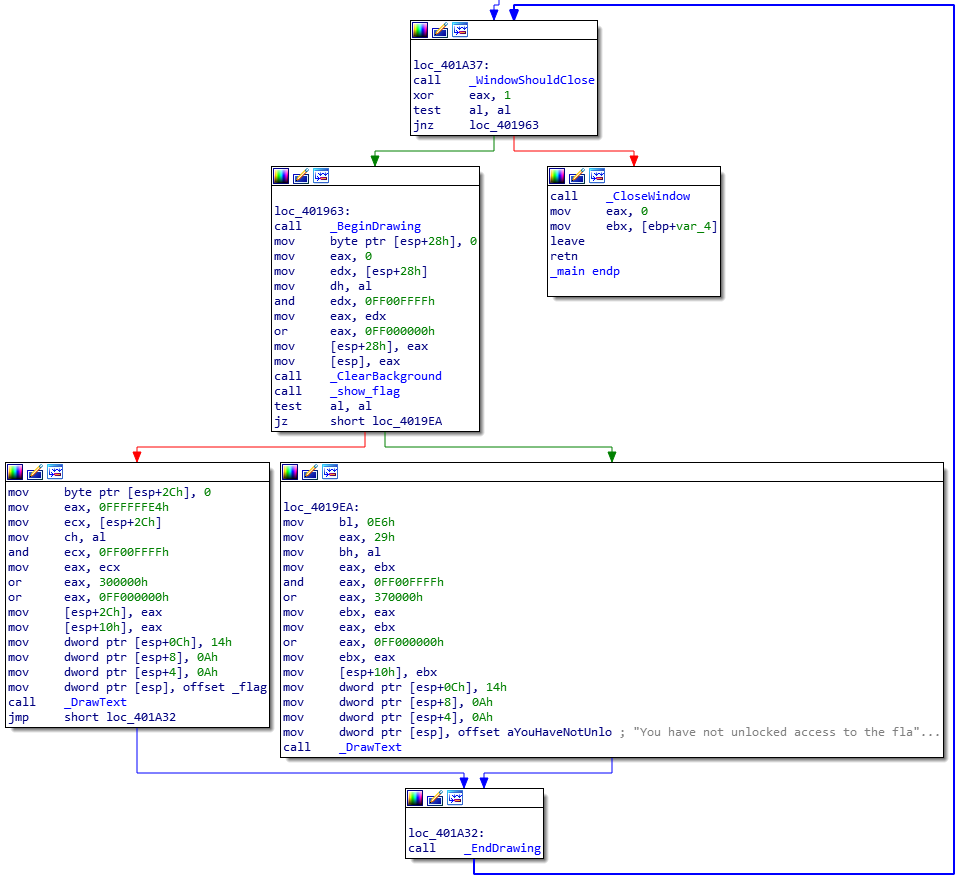
\includegraphics[width=16cm]{200_ida_graph}
    \caption{Widok grafowy w programie IDA przestawiający główną pętle programu}
    \label{fig:200_ida_graph}
\end{figure}

Zauważa on, że wywołanie funkcji o nazwie \emph{\_show\_flag} decyduję o wyborze jednego
z dwóch węzłów wywołania programu. Biorąc pod uwagę nazwę tej funkcji oraz tekst
wyświetlany w prawym węźle (\textit{,,You have not unlocked access to the fla''...}), domyśla
się, że funkcja \emph{\_show\_flag} decyduję o tym czy flaga zostanie wyświetlona użytkownikowi.

\begin{figure}[H]
    \centering
    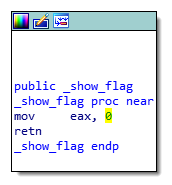
\includegraphics{200_ida_show_flag}
    \caption{Funkcja \emph{\_show\_flag}}
    \label{fig:200_ida_show_flag}
\end{figure}

Jedyne co ta funkcja robi to zwraca liczbę 0 -- czyli \emph{false}.
Próbuję on więc spatchować\footnote{Patchowanie w tym wypadku oznacza modyfikowanie programu
wykonywalnego poprzez nadpisanie konkretnych bajtów}
program, aby funkcja ta zwracała 1 -- czyli \emph{true}.

\begin{figure}[H]
    \centering
    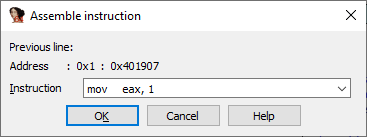
\includegraphics{200_ida_patch}
    \caption{Modyfikacja instrukcji, aby zwracała 1 zamiast 0}
    \label{fig:200_ida_patch}
\end{figure}

Po zaaplikowaniu patch'a oraz ponownym uruchomieniu programu użytkownikowi ukazuję się
następujący widok.

\begin{figure}[H]
    \centering
    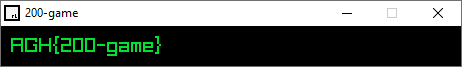
\includegraphics{200_flag}
    \caption{Okienko programu wraz z otrzymaną flagą}
    \label{fig:200_flag}
\end{figure}

Po wpisaniu na stronie flagi \emph{AGH\{200-game\}} użytkownik otrzymuję informację
o poprawnym rozwiązaniu zadania.

\clearpage

\subsection{Zadanie 300-strcmp}

Użytkownik pobiera plik \emph{strcmp} i sprawdza go programem \emph{file}.

\begin{minted}[breaklines]{text}
$ file strcmp
strcmp: ELF 64-bit LSB pie executable, x86-64, version 1 (SYSV), dynamically linked, interpreter /lib64/ld-linux-x86-64.so.2, BuildID[sha1]=bda67999b52d8f4d1f9456346119790c47c261d8, for GNU/Linux 3.2.0, stripped
\end{minted}

Dowiaduje się, że jest to 64-bitowy plik wykonywalny na platformę Linux.
Uruchamia więc go, aby sprawdzić jego działanie.

\begin{minted}{text}
$ ./strcmp
Enter the flag: test
Incorrect flag!
\end{minted}

Aby przeanalizować działanie programu otwiera go w darmowym narzędziu dostępnym przez
przeglądarkę Binary Ninja Cloud\footnote{Binary Ninja Cloud: \url{https://cloud.binary.ninja/}}.

\begin{figure}[H]
    \centering
    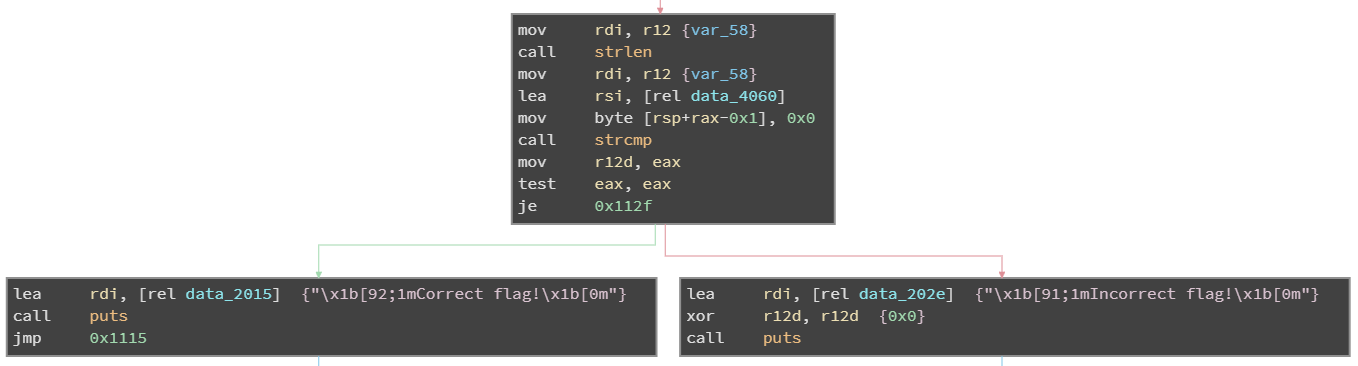
\includegraphics[width=16cm]{300_binary_ninja}
    \caption{Widok grafowy w programie Binary Ninja Cloud}
    \label{fig:300_binary_ninja}
\end{figure}

Zauważa, że za sprawdzenie poprawności flagi odpowiada funkcja \emph{strcmp}, która
jako jednego z argumentów używa niemodyfikowanego wejścia użytkownika.
Oznacza to, że flaga również musi być przekazana w jawnej formie do tej funkcji.
Korzysta on więc z GNU Debugger, aby odczytać przekazany do niej drugi parametr.

\begin{minted}{text}
$ gdb -q strcmp
Reading symbols from strcmp...
(No debugging symbols found in strcmp)
(gdb) info functions strcmp
All functions matching regular expression "strcmp":

Non-debugging symbols:
0x0000000000001080  strcmp@plt
\end{minted}

Zakłada teraz punkt przerwania w momencie wywołania funkcji \emph{strcmp}.

\begin{minted}{text}
(gdb) break strcmp@plt
Breakpoint 1 at 0x1080
\end{minted}

Uruchamia program i wpisuje dowolny tekst, aby przejść do punktu przerwania.

\begin{minted}{text}
(gdb) run
Starting program: /home/piotr/strcmp 
Enter the flag: test

Breakpoint 1, 0x0000555555555080 in strcmp@plt ()
\end{minted}

Kiedy program zatrzyma się w pożądanym miejscu, użytkownik podgląda zawartość pamięci na którą
zgodnie z konwencją wywołania System V AMD64\footnote{
\url{https://en.wikipedia.org/wiki/X86_calling_conventions\#System_V_AMD64_ABI}}
wskazują rejestry RDI oraz RSI - czyli dwa parametry przekazane do funkcji \emph{strcmp}.

\begin{minted}{text}
(gdb) x/s $rdi
0x7fffffffe620:	"test"
(gdb) x/s $rsi
0x555555558060:	"AGH{300-strcmp}"
\end{minted}

W rejestrze RDI znajduję się adres tekstu wpisanego przez użytkownika, natomiast
w rejestrze RSI ciąg znaków, z którym wejście od użytkownika jest porównywane -- czyli
jawna postać flagi. W taki sposób użytkownik otrzymuję flagę \emph{AGH\{300-strcmp\}},
która jest rozwiązaniem tego zadania.
\clearpage

\subsection{Zadanie 400-decrypt}

Użytkownik pobiera plik \emph{decrypt} i podobnie jak wcześniej sprawdza go programem \emph{file}.

\begin{minted}[breaklines]{text}
$ file decrypt
decrypt: ELF 64-bit LSB pie executable, x86-64, version 1 (SYSV), dynamically linked, interpreter /lib64/ld-linux-x86-64.so.2, BuildID[sha1]=8b4924f98f391fb9939f323d9a89e37d2e7febb7, for GNU/Linux 3.2.0, not stripped
\end{minted}

Podobnie jak w poprzednim zadaniu, dowiaduję się, że jest to 64-bitowy linuksowy program.
Uruchamia go.

\begin{minted}{text}
$ ./decrypt
Enter the flag: test
Incorrect flag!
\end{minted}

Tym razem do analizy programu użyje narzędzia Ghidra\footnote{\url{https://ghidra-sre.org/}}.
Potrafi ona generować pseudokod na podstawie kodu maszynowego programu, co bardzo ułatwia
analizowanie plików wykonywalnych.
Użytkownik wczytuje pobrany plik wykonywalny do narzędzia, a następnie korzystając z funkcji
zmiany nazw symboli, zmienia nazwy zmiennych tam gdzie jest to dla niego oczywiste.
Otrzymuje on następujący fragment pseudokodu.

\begin{minted}{c}
    sVar3 = strlen(input);
    length = (int)sVar3 + -1;
    input[length] = '\0';
    if (length == 0x10) {
      encrypt(input,0x10);
      same = true;
      i = 0;
      while (i < 0x10) {
        if (input[i] != flag[i]) {
          same = false;
          break;
        }
        i = i + 1;
      }
      if (same) {
        puts("\x1b[92;1mCorrect flag!\x1b[0m");
        uVar2 = 0;
        goto LAB_001013da;
      }
    }
    puts("\x1b[91;1mIncorrect flag!\x1b[0m");
    uVar2 = 0;
\end{minted}

Zauważa, że powyższy fragment kodu szyfruje tekst wprowadzony przez użytkownika,
a następnie porównuje go z ciągiem znaków zawartym w zmiennej \emph{flag}.
Zmienna flag okazuje się tablicą 16 elementów:
\emph{90 f9 eb 94 ea 9d 8e c2 af df ce 8a b2 ce d9 92}.

Następnie analizuje pseudokod funkcji \emph{encrypt} zmieniając nazwy zmiennych
dla poprawy czytelności.

\begin{minted}{c}
void encrypt(char *input,int length)
{
...
  i = 0;
  while (i < length) {
    c = input[i];
    if ((c < 'A') || ('Z' < c)) {
      if (('`' < c) && (c < '{')) {
        if (c < 'n') {
          input[i] = c + '\r';
        }
        else {
          input[i] = c + -0xd;
        }
      }
    }
    else {
      if (c < 'N') {
        input[i] = c + '\r';
      }
      else {
        input[i] = c + -0xd;
      }
    }
    i = i + 1;
  }
  key = 0xefbeadde;
  k = 0;
  j = 0;
  while (j < length) {
    input[j] = key[k] ^ input[j];
    k = k + 1U & 3;
    j = j + 1;
  }
}
\end{minted}

Zauważa, że funkcja szyfrująca dzieli się na dwa fragmenty.
Pierwszy fragment przechodzi po każdym znaku tablicy wejściowej i dodaje
\emph{'\textbackslash r'} lub
odejmuje \emph{0xd} w zależności czy dany znak spełnia warunki.
Zarówno \emph{'\textbackslash r'} jak i \emph{0xd} to 13 w systemie dziesiętnym.
Analizując warunki dochodzi do wniosku, że jest to prosty szyfr przesuwający zwany ROT13.
Drugi fragment również przechodzi po każdym znaku tablicy, a następnie wykonuje
operacje XOR z kolejnymi bajtami klucza (wracając do pierwszego bajtu po ostatnim).
Biorąc pod uwagę, że liczby całkowite przechowywane
są w pamięci w formie Little Endian, to klucz również można zapisać następująco:
\emph{0xDE, 0xAD, 0xBE, 0xEF}.

Posiadając te informacje pisze skrypt w języku Python, który odwróci wcześniej otrzymaną
tablice \emph{flag} do wartości pierwotnej.

\begin{minted}[breaklines]{python}
flag = [0x90, 0xF9, 0xEB, 0x94, 0xEA, 0x9D, 0x8E, 0xC2, 0xAF, 0xDF, 0xCE, 0x8A, 0xB2, 0xCE, 0xD9, 0x92]

# XOR cipher
key = [0xDE, 0xAD, 0xBE, 0xEF]
for i in range(len(flag)):
    flag[i] ^= key[i % len(key)]

# ROT13
for i in range(len(flag)):
    c = flag[i]

    if c >= ord("A") and c <= ord("Z"):
        if c + 13 <= ord("Z"):
            flag[i] = c + 13
        else:
            flag[i] = c - 13
    elif c >= ord("a") and c <= ord("z"):
        if c + 13 <= ord("z"):
            flag[i] = c + 13
        else:
            flag[i] = c - 13


print("".join([chr(x) for x in flag]))
\end{minted}

Zapisuje skrypt jako \emph{decrypt.py} i uruchamia go.

\begin{minted}{text}
$ python decrypt.py
AGH{400-decrypt}
\end{minted}

Otrzymuje rozwiązanie tego zadania, czyli flagę \emph{AGH\{400-decrypt\}}.
\clearpage

\subsection{Zadanie 500-secret-shell}

\subsection{Zadanie 600-custom-vm}

\end{document}
